%reset references counter
\setcounter{NAT@ctr}{-1}
\cleartorightpage
\chapter*{}\label{chapter:galaxy}
\phantomsection\addcontentsline{toc}{section}{Galaxy: the 2018 update}

\begin{figure}[t!]
\centering

\includegraphics[height=10em]{frontmatter/images/chapter-header-galaxy.png}
\end{figure}
\vspace{-4cm}

\begin{changemargin}{0cm}{2cm}
\articletitle{The Galaxy platform for accessible, reproducible and collaborative biomedical analyses: 2018 update}
\end{changemargin}


Enis Afgan\textsuperscript{\ref{affil:hopkins},*},
Dannon Baker\textsuperscript{\ref{affil:hopkins}},
Bérénice Batut\textsuperscript{\ref{affil:freiburg},*},
Marius van den Beek\textsuperscript{\ref{affil:curie},*},
Dave Bouvier\textsuperscript{\ref{affil:pennstate},*},
Martin Čech\textsuperscript{\ref{affil:pennstate},*},
John Chilton\textsuperscript{\ref{affil:pennstate},*},
Dave Clements\textsuperscript{\ref{affil:hopkins},*},
Nate Coraor\textsuperscript{\ref{affil:pennstate},*},
Björn Grüning\textsuperscript{\ref{affil:freiburg},*},
Aysam Guerler\textsuperscript{\ref{affil:hopkins},*},
Jennifer Hillman-Jackson\textsuperscript{\ref{affil:pennstate},*},
Saskia Hiltemann\textsuperscript{\ref{affil:emc},*},
Vahid Jalili\textsuperscript{\ref{affil:oregon},*},
Helena Rasche\textsuperscript{\ref{affil:freiburg},*},
Nicola Soranzo\textsuperscript{\ref{affil:earlham}},
Jeremy Goecks\textsuperscript{\ref{affil:oregon},*},
James Taylor\textsuperscript{\ref{affil:hopkins},*},
Anton Nekrutenko\textsuperscript{\ref{affil:pennstate},*},
Daniel Blankenberg\textsuperscript{\ref{affil:cleveland},*}

* The authors wish it to be known that, in their opinion, all authors should be regarded as Joint First Authors.

\textbf{Published in:} \emph{Nucleic Acids Research}, Volume 46, Issue W1, 2 July 2018, Pages W537–W544,  \\
DOI: \url{https://doi.org/10.1093/nar/gky379}

\small
\begin{enumerate}
\itemsep-0.5em
\item Department of Biology, Johns Hopkins University, Baltimore MD USA.\label{affil:hopkins}
\item Department of Comuter Science, Albert-Ludwigs-University, Freiburg, Germany.\label{affil:freiburg}
\item Institut Curie, PSL Research University, Paris, France.\label{affil:curie}
\item Department of Biochemistry and Molecular Biology, Penn State University, University Park, PA, USA.\label{affil:pennstate}
\item Center for Biological Systems Analysis (ZBSA), University of Freiburg, Freiburg, Germany.\label{affil:freiburg2}
\item Department of Pathology, Erasmus Medical Centre, Rotterdam, The Netherlands.\label{affil:emc}
\item Department of Biomedical Engineering, Oregon Health and Science University, OR, USA.\label{affil:oregon}
\item Earlham Institute, Norwich Research Park, Norwich, United Kingdom.\label{affil:earlham}
\item Genomic Medicine Institute, Lerner Research Institute, Cleveland Clinic, Cleveland, OH, USA.\label{affil:cleveland}
\end{enumerate}
\normalsize


\section*{Abstract}
Galaxy (homepage: \url{https://galaxyproject.org}, main public server: \url{https://usegalaxy.org}) is a web-based scientific analysis platform used by tens of thousands of scientists across the world to analyze large biomedical datasets such as those found in genomics, proteomics, metabolomics, and imaging. Started in 2005, Galaxy continues to focus on three key challenges of data-driven biomedical science: making analyses accessible to all researchers, ensuring analyses are completely reproducible, and making it simple to communicate analyses so that they can be reused and extended. During the last two years, the Galaxy team and the open-source community around Galaxy have made substantial improvements to Galaxy’s core framework, user interface, tools, and training materials. Framework and user interface improvements now enable Galaxy to be used for analyzing tens of thousands of datasets, and more than 5,500 tools are now available from the Galaxy ToolShed. The Galaxy community has led an effort to create numerous high-quality tutorials focused on common types of genomic analyses. The Galaxy developer and user communities continue to grow and be integral to Galaxy’s development. The number of Galaxy public servers, developers contributing to the Galaxy framework and its tools, and users of the main Galaxy server have all increased substantially.


\section*{Introduction}
Advances in biomedicine and biology increasingly rely on analysis of large datasets. Started in 2005, the Galaxy Project (\url{https://galaxyproject.org})~\cite{giardine2005galaxy,blankenberg2007framework,afgan2016galaxy} maintains a focus on enabling data-driven biomedical science by pursuing three goals: (a) accessible data analysis serving all scientists regardless of their informatics expertise and tool developers seeking a wider audience and broad integration of their tools; (b) reproducible analyses regardless of the particular platform; and (c) transparent communication of analyses, which in turn enables reuse and extension of analyses across communities of practice. The Galaxy Project consists of four complementary components:

\begin{enumerate}
\item The main public Galaxy server (\url{https://usegalaxy.org}) — this server is the subject of this article and has been online since 2007. It features a rich toolset for large-scale genomics analyses, terabytes of public data for use, and hundreds of shared analysis histories, workflows, and interactive publication supplements. This server has more than 124,000 registered users whom run \~245,000 analysis jobs each month.

\item The Galaxy framework and software ecosystem (\url{https://github.com/galaxyproject}) — an open-source software package that anyone can use to run a Galaxy server on any Unix-based operating system. The Galaxy ecosystem includes a software development kit (SDK) for Galaxy tool development, API language bindings for multiple programming languages, software for scripting Galaxy interactions, and tools for automating setup and deployment of Galaxy and its plugins such as tools and visualizations.

\item The Galaxy ToolShed (\url{https://toolshed.g2.bx.psu.edu/}) — a community-driven resource for the dissemination of Galaxy tools, workflows, and visualizations. This server functions as an “AppStore” for Galaxy servers where developers and Galaxy admins can host, share, and install Galaxy tools, workflows, and visualizations.

\item The Galaxy Community (\url{https://galaxyproject.org/community/}) — distinct and complementary subcommunities make key contributions to all aspects of the Project. These subcommunities address the needs and desires of every category of stakeholder including users, administrators, developers, resource providers, and educators.
\end{enumerate}

Galaxy has served hundreds of thousands of users, been used in more than 5,700 scientific publications, and provided 500+ developers with a framework provisioning accessible, transparent, and reproducible data analysis (\url{https://galaxyproject.org/galaxy-project/statistics/}). Many instances of the framework have been installed, including Galaxy Main (\url{https://usegalaxy.org}) and over 99 publicly accessible servers (\url{https://galaxyproject.org/public-galaxy-servers/}), serving biomedical and other domain-specific research. Significant growth has occurred across all sectors of the Galaxy Project within the past two years (\hyperref[fig:growth]{Fig.~\ref{fig:growth}}).


\begin{figure}[ht!]
\centering
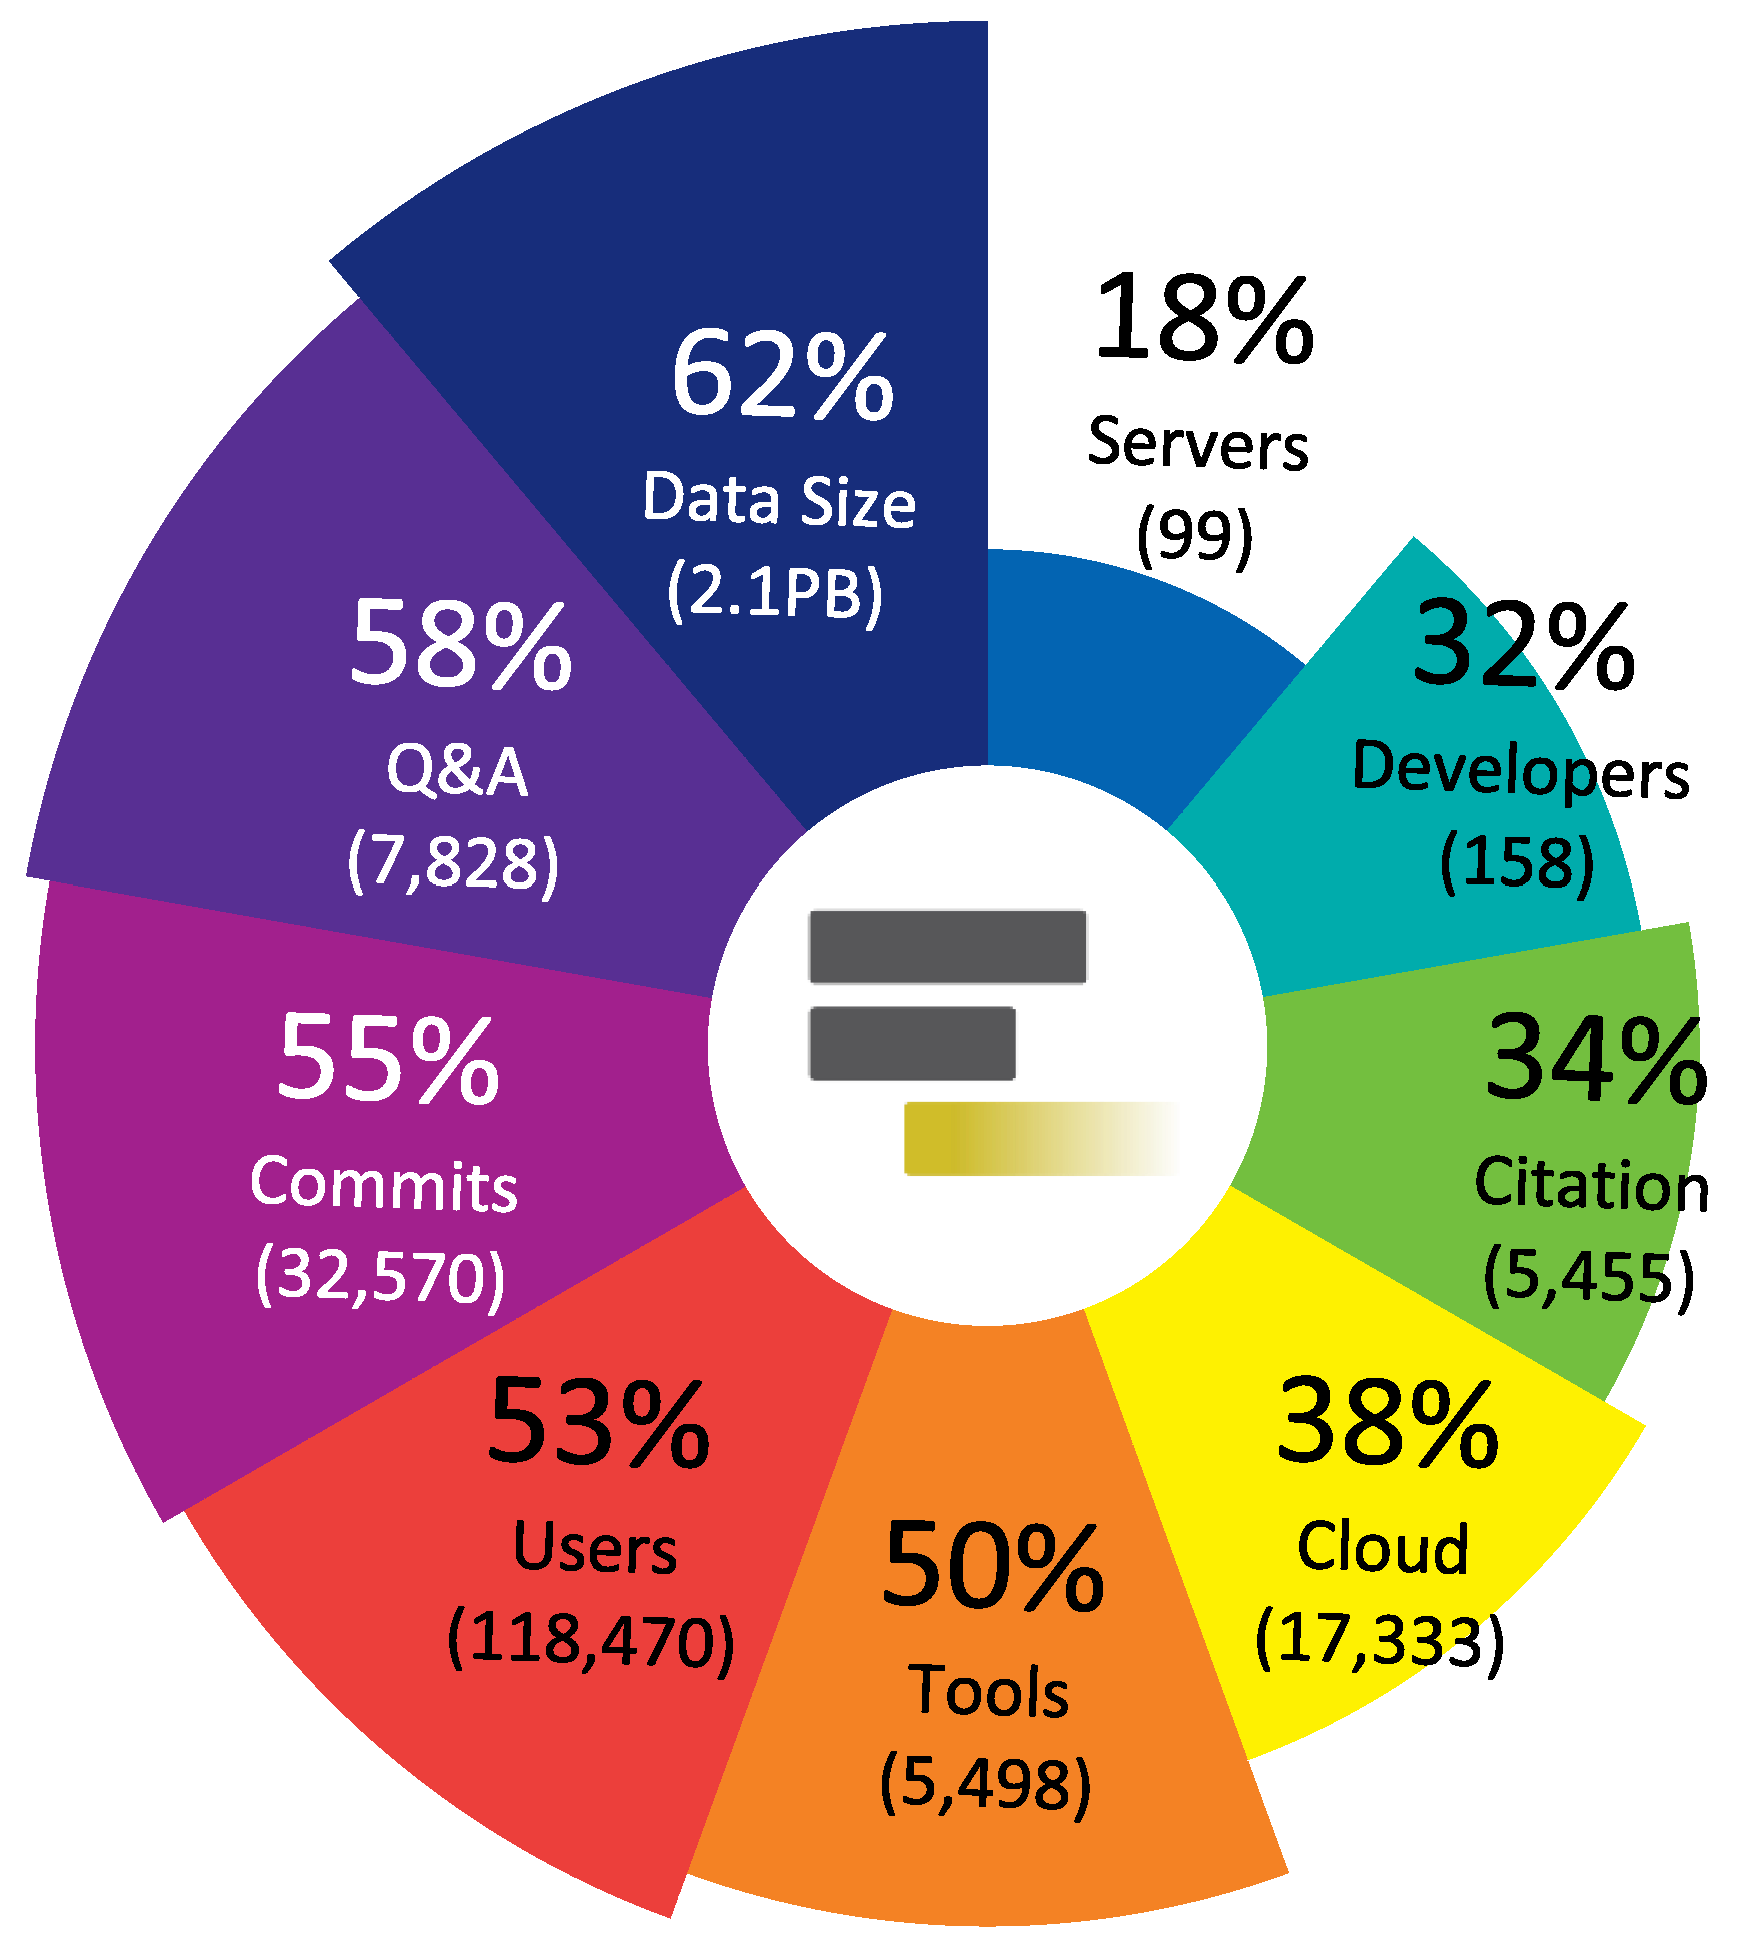
\includegraphics[]{chapters/images/galaxy/galaxy-growth.png}
\caption{Circular barplot illustrating recent growth of the Galaxy Project across several independent facets. In the past two years, usage of the main public Galaxy server has increased 60\%, the number of tools and supported versions has increased 53\%, and the amount of data analyzed on the main server has increased 72\%. A growing number of public instances (18\% increase) and cloud-based Galaxies (38\% increase) provide researchers with a wider range of options for scalability and application domains. Additionally, more developers (45\% increase with 63\% more commits to the codebase) contributed to the Galaxy framework and software ecosystem. Question and answer activity on the Galaxy Biostars forum increased 68\%.}
\label{fig:growth}
\end{figure}

\section*{New Features}
\subsection*{Scalability}
Scalability is amongst the most significant challenges that Galaxy faces as the size and number of biomedical and especially genomics datasets continues to grow. For instance, single-cell RNA-seq experiments routinely generate hundreds or thousands of primary datasets. As a web-based application, Galaxy must scale both in its web-based interface and on its backend server and do so in a multiuser environment.

\paragraph*{User interface scalability} enables scientists to use the Galaxy web interface to analyze many datasets, apply (collective) operations on them, and design pipelines to analyze them. Galaxy implements a variety of features to facilitate analyzing large numbers of datasets, including workflows and collections. Our recent optimizations of the user interface (UI) yielded a significant improvement to frontend scalability. We benchmarked the optimizations by replicating an experiment conducted on single Hematopoietic stem cells and multipotent progenitors~\cite{yang2016single} to quantify the expression of 64,000 transcripts, which generates 11,872 history items. Galaxy ran this proof of concept experiment seamlessly using existing standard tools, whereas earlier versions of Galaxy would not have been able to support this analysis.

\paragraph*{Server scalability} refers to the Galaxy’s ability to execute many data analysis/manipulation tasks for many users. This is achieved by advantageously utilizing a range of available computing resources. The Galaxy framework runs on various platforms, from a standard laptop to institutional clusters and cloud-based platforms. Galaxy is highly versatile in its ability to deploy jobs (atomic units of work), as it can leverage a multitude of workload managers including Slurm~\cite{yoo2003slurm}, HTCondor~\cite{thain2005distributed}, Apache Mesos~\cite{hindman2011mesos}, and Kubernetes (\url{https://kubernetes.io}), among others, in addition to a built-in lightweight job running system. Recent enhancements to Galaxy’s job management include dynamic job destination assignment (which facilitate automatic job parameter-specific resource selection), delay in job queuing (e.g., for workflows), automatic job re-submission (e.g., on job failure due to a temporary cluster error), and means of implementing fair-share prioritization schemes. These features are being used on Galaxy Main (\hyperref[fig:setup]{Fig.~\ref{fig:setup}}) to leverage cloud computing resources for better job throughput. Specifically, Galaxy Main is now configured to take advantage of the XSEDE infrastructure~\cite{towns2014xsede} that includes Bridges and Stampede resources as well as the Jetstream cloud~\cite{stewart2015jetstream}. The benefits of using these resources include the ability to run larger jobs, as shown in \hyperref[fig:infra]{Figure~\ref{fig:infra}}. Additionally, use of these resources has enabled new types of analysis to be enabled on Main. Notably, this includes Galaxy Interactive Environments through to the ability to use containerization technologies and provide sufficient isolation of individual jobs from other processes running on the same underlying compute infrastructure.

\begin{figure}[t!]
\centering
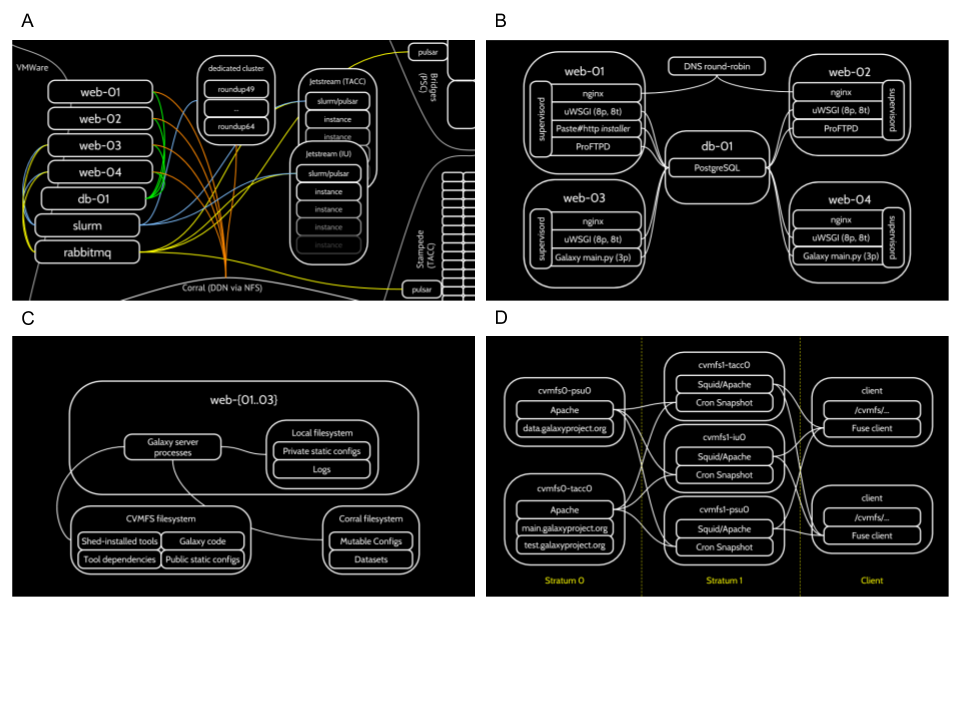
\includegraphics[width=\textwidth]{chapters/images/galaxy/setup.png}
\caption{Schematic of servers and services in use at Galaxy Main. (A) A global overview of Galaxy Main resources. (B) Multiple frontend servers serve Galaxy content to users by utilizing round-robin load balancing. (C) Layout of data schemes used by Galaxy Main is optimized for application speed, concurrent access, and versioned content. (D) CVMFS infrastructure hosted by the Galaxy Project that is used at Main and available for access to any other Galaxy instance.}
\label{fig:setup}
\end{figure}

\begin{figure}[t!]
\centering
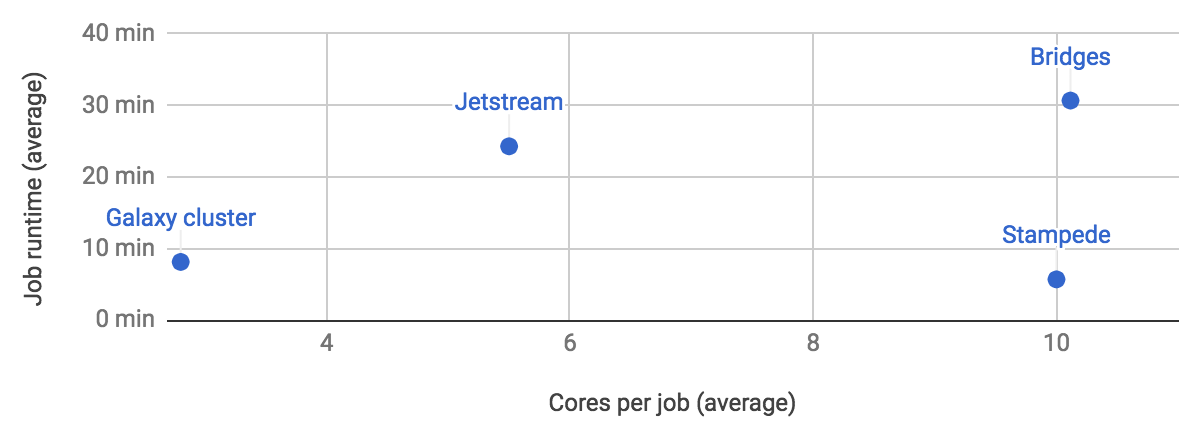
\includegraphics[width=\textwidth]{chapters/images/galaxy/infra.png}
\caption{Enabling automated selection and use of specialized national cyberinfrastructure compute resources from Galaxy Main enhances user-experience. It is now possible to run jobs that are up to an order of magnitude larger than before by using Bridges and Stampede. New types of jobs, such as interactive environments (see Advances in tools section), that require execution isolation due to security concerns are enabled by utilizing virtualization facilitated by the Jetstream cloud. Consequently, it is possible to concurrently run more jobs due to the increase in processing capacity.}
\label{fig:infra}
\end{figure}

A complete Galaxy server with a full repertoire of tools and reference data can be run on major cloud platforms. These servers are launched independently by users, and come pre-configured with hundreds of tools and reasonable default settings typical of a production server. Notably, launched instances do not have usage quotas and can be customized to install any desired tool. We have designed a cloud-agnostic approach for leveraging these resources by developing the abstraction library CloudBridge~\cite{goonasekera2016cloudbridge} and a new CloudLaunch application. These two solutions make it possible to launch Galaxy instances across a variety of cloud providers while reducing the requirement to build and maintain cloud-specific resources (e.g., machine images, file systems). There are now ten different flavors of Galaxy available for launching on major clouds including Amazon Web Services, Jetstream, and Microsoft Azure (\url{https://launch.usegalaxy.org}).

\subsection*{Advances in tools}
The Galaxy ToolShed~\cite{blankenberg2014dissemination} assumes the role of an AppStore for Galaxy instances by hosting thousands of tools. The ToolShed improves tool availability, deployment, and portability across Galaxy servers and computing environments.

\paragraph*{Updated tool suite} Over the last two years, we have expanded both the quantity and quality of the tools available on the Galaxy Toolshed. As of April 2018, the ToolShed hosts 5,628 tools, which shows 53\% growth since 2016, and approximately 2,000 repositories had at least one new update. Examples of new tools include: GEMINI for exploring genetic variation~\cite{paila2013gemini}; mothur for analyzing rRNA gene sequences~\cite{schloss2009introducing}; QIIME for quantitative microbiome analysis from raw DNA sequencing data~\cite{caporaso2010qiime}; deepTools for explorative analysis of deeply sequence data~\cite{ramirez2014deeptools,ramirez2016deeptools2}; HiCexplorer~\cite{ramirez2018high} for analysis and visualization of Hi-C data; ChemicalToolBox for comprehensive access to cheminformatics libraries and drug discovery tools~\cite{lucas2014chemicaltoolbox}; minimap2 (\url{https://arxiv.org/abs/1708.01492}) and poretools for long read sequencing analysis~\cite{loman2014poretools}; MultiQC~\cite{ewels2016multiqc} to aggregate multiple results into a single report; a new RNA-seq analysis tool suite with modern analysis tools such as Kallisto~\cite{bray2016near}, Salmon~\cite{patro2017salmon}, Deseq2~\cite{love2014moderated}, and STAR-Fusion~\cite{dobin2013star}; and GenomeSpace~\cite{qu2016integrative}, a cloud-based interoperability tool.

\paragraph*{Tool environment and interface.}
The portability and backward-compatibility of the Galaxy tools environment is improved significantly. Accordingly, a tool configuration now includes a tool profile version, which is used to ensure compatibility between a version of a tool and its targeted Galaxy version. In addition, tool profile versions allow for the evolution of new and better tool defaults and behaviors while maintaining backwards compatibility. We also improved the ToolShed API and its interface to facilitate installing tools missing from an imported workflow. We improved the installation process so that restarting Galaxy is not required to use a newly installed tool.

\subsection*{Interactive analysis and visualization}
Galaxy’s UI makes it possible for anyone to run complex analyses. However, a complete analysis of genomic data often requires custom scripts or visualizations, especially at the beginning (data preparation) or end (data summarization) of analyses. To meet these customized needs, we recently introduced Galaxy Interactive Environments~\cite{gruning2017jupyter}, an integration of Galaxy with Jupyter (RStudio is in development)—a commonly used interactive scripting platform. With Interactive Environments, Galaxy users benefit from existing computational infrastructure via both graphical UI and ad hoc scripting, or any combination of these.

Galaxy’s visualization framework~\cite{goecks2013web} makes it possible to integrate a wide variety of Web-based and server-side visualizations. Through this framework, many new visualizations have been added to Galaxy, including Cytoscape~\cite{shannon2003cytoscape}, and the WebGL enabled 3D Protein viewer NGL~\cite{rose2015ngl}, molecular interaction networks and macromolecular structures visualizations, and the 100+ visualizations available through BioJS~\cite{gomez2013biojs}, a rich set of community-driven JavaScript components for agile and interactive visualization of biological data.

\subsection*{User interface and experience enhancements}
There are two common modes of data analysis: exploratory and pipeline execution. Galaxy enables simultaneous access to both of these. Users are able to interactively analyze their data by making use of individual tools in a trial-and-error manner. They are then able to automatically generate reusable and generalizable workflows from an ad hoc analysis. An interactive workflow editor is also available to modify or generate workflows from scratch. At any point in time, a user can seamlessly switch modes between interactively analyzing a datasets and executing a workflow on these datasets. There is no analysis lock-in, and users can exercise full control, or make use of pre-existing pipelines. Importantly, these analysis artefacts, such as datasets, analysis histories, workflows, and visualizations can all be shared and copied by collaborators at the discretion of the analyst.

\paragraph*{Client-side infrastructure}
The client-side of Galaxy, which is the user-interface most people associate Galaxy with, has seen significant changes under the hood. The usage of server-side mako templates, for example to create forms, has been further reduced and replaced by client-side only code that communicates via the RESTful Galaxy API with the backend. This minimizes the number of full-page refreshes and improves response time by enabling partial page updates. The interface has been further enhanced to allow for drag-and-drop of files and datasets, presents a fuzzy search on dataset and tool metadata, and implements a modal scratchbook for visualizations and comparison of multiple datasets.

Furthermore, the community has selected the Vue.js framework (\url{https://vuejs.org/}) as the base for future improvements allowing all UI elements to converge into a more reactive and future-proof interface. With the integration of Vue.js, the entire client-side build system was updated to utilize the latest web-technologies, to make routing and loading times faster, and to encourage rapid future interface improvements. While mostly transparent to users, these changes are the fundamental groundwork of a more more flexible UI framework that will enable visual enhancements and an improved user experience for years to come.

\paragraph*{Tags.}
Although tags have been supported in Galaxy for several years, they have only recently become advantageous for large many-sample analyses. We have enhanced tags to allow propagation through dataset analysis steps. This facilitates tracking individual datasets through the entire analysis life-cycle and becomes part of the provenance system and ease-of-use of Galaxy. To enable automatic tag propagation, a hash-sign (\#) is placed at the beginning of the tag, which is colloquially referred to as a named-tag. While standard Galaxy output dataset naming is suitable for many interactive analyses, the connection between inputs and outputs through large workflows becomes increasingly less obvious; by utilizing named-tags, users can label datasets with an identifier that is maintained throughout the analysis.

\paragraph*{Webhooks.}
Inspired by user feedback and the need to quickly modify and adapt Galaxy’s interface, we integrated a pluggable system to extend Galaxy’s frontend. Webhooks provide an entry-point into the Galaxy UI, in which it is possible to add buttons, menu entries, or entire iframes. At these entry-points a developer can dynamically add client-side code (JavaScript, HTML, CSS) and interact with the rest of the Galaxy user-interface. By integrating Webhooks with the Galaxy API, it is also possible to trigger server-side functions from within a Webhook. Webhooks can be thoroughly customized and are enabled at the discretion of the Galaxy administrator.

\paragraph*{Interactive tours.}
We have developed self-paced, interactive tours that users can step through to learn about Galaxy. These tours guide users step by step through using the interface including tools, workflows, and other features available in Galaxy. To simplify tour creation, a Tour Builder (\url{https://github.com/TailorDev/galaxy-tourbuilder}) has been created for recording, replaying, updating, and exporting tours.

\paragraph*{Improved workflows.}
Galaxy workflows have been extended in several ways. Switching between tool versions and upgrading workflows with new tool versions is now supported. A workflow can now be embedded in another, making it easier to create and edit workflows that have many common steps repeated. Many of these features have existed in in standalone workflow systems, such as Taverna~\cite{wolstencroft2013taverna}, for sometime, but have been widely requested by Galaxy users. Workflows are now scheduled by a Galaxy server more efficiently and in the background, making it possible to execute larger workflows, generating tens of thousands of jobs, while providing instant feedback and a snappier user-experience. We have also enhanced Galaxy with initial support for running workflows defined in the Common Workflow Language~\cite{amstutz2016common} format.

\paragraph*{Dataset collections}
Galaxy Dataset Collections combine datasets to enable simultaneous analysis. They organize sets of datasets as potentially nested lists of objects allowing easier data handling and batch execution of tools. In addition to the related frontend improvements, and support of nesting collections together, we recently introduced specialized tools to be executed on collections (e.g., Collapse, which combines a list of datasets into a single dataset, Flatten which takes nested collections and produces a flat list of datasets, and Merge which takes two lists and creates a single unified list), and enabled uploading and downloading dataset collections to and from both user’s local disk and Galaxy data libraries.

\subsection*{Infrastructure enhancements}
In order to make Galaxy more robust in a production environment, we adopted technologies to enhance Galaxy’s portability, security, reliability, and scalability. Galaxy now utilizes uWSGI (\url{http://projects.unbit.it/uwsgi}) as its default web application server. This adoption has several advantages, namely the ability to negate Python’s limitations regarding concurrent tasks execution, built-in load balancing, scalability, improved fault tolerance, and the possibility of restarting Galaxy uninterruptedly.

Many tools available via Galaxy rely on the availability of reference and index data. To promote ease of use and efficient storage and compute resources, Galaxy is able to share a precomputed set of local reference data for tools to use. Previously, making this data available to the tools was a time intensive process where a Galaxy administrator had to install and properly configure the server, either manually or by using Data Managers~\cite{blankenberg2014wrangling}. However, this resulted in much redundant effort required for each Galaxy server being configured. To streamline this process, we have made all the reference data we prepared for Galaxy Main available via a CernVM File System~\cite{blomer2012status}, a scalable and content-addressable file system. This repository currently hosts 5TB of pre-build reference data, which are versioned and shared publicly with read-only access. With minimal configuration, any instance of Galaxy, including Galaxy-Docker images, can attach to this file system and gain access to the same reference data available on Galaxy Main. To improve accessibility and fault-tolerance, this data source is replicated on servers located in Europe and Australia.

Galaxy is powered by various open-source projects which are installed automatically, and used when needed. Galaxy is using the Conda package manager (\url{https://conda.io}) as its default tool dependency resolver, and offers support for virtualization and containerization technologies (e.g., Docker (https://www.docker.com) and Singularity~\cite{kurtzer2017singularity}) to ensure a higher level of portability, if needed. By leveraging the Bioconda (\url{https://doi.org/10.1101/207092}) and the BioContainer~\cite{da2017biocontainers} projects, Galaxy is able to provision and use reproducible tool execution environments.

Galaxy is a generic data analysis framework, which can be configured for various application scenarios using a wide range of configuration parameters. To facilitate configuring these parameters with optimal values for a number of predefined application scenarios, the Galaxy project leverages Ansible (\url{https://www.ansible.com}), software for automated configuration and management of other software packages. We have developed and shared Ansible configurations for Galaxy Main, the main public Galaxy server, (\url{https://github.com/galaxyproject/usegalaxy-playbook}) and also a configurable generic playbook for setting up production instances on cloud resources, virtual machines, and bare metal (\url{https://github.com/ARTbio/GalaxyKickStart}). This playbook can be used as a reference for configuring a Galaxy instance for a production environment.

The Galaxy-Docker project (\url{https://github.com/bgruening/docker-galaxy-stable}), delivers a production ready Galaxy instance in minutes and can be used as the basis for personalised, self-contained, portable instances of Galaxy, known as Galaxy flavors. Preconfigured by the Galaxy community a plenitude of flavors already exist covering application scenarios, from BLAST+~\cite{cock2015ncbi,camacho2009blast+}, metagenomics (\url{https://doi.org/10.1101/183970}), ChIP-exo analysis, or RNA research~\cite{gruning2017rna}. In addition to the facilitated and out-of-box functionality, these images provision isolated environments well-suited for experimenting with tools and Galaxy configurations, and are ideal for training courses, as demonstrated by the Galaxy Training Network.

Server monitoring and issue management is crucial in production Galaxy instances. Galaxy has integrated a plugin module to submit user bug-reports to configurable endpoints such as mailing lists or GitHub issues. With this, Galaxy can be configured to send error reports to a local ticket system. The recent integration of Sentry (\url{https://sentry.io/}) for automated error tracking and reporting makes it easier for administrators to track both client- and server-side errors without requiring manual user bug reports.

\section*{Community}
Galaxy serves several distinct communities: researchers, tool developers, resource providers, trainers, and trainees. To centralize resources for all communities, we have developed the The Galaxy Community Hub (\url{https://galaxyproject.org}) for all things Galaxy. The Hub uses a modified wiki approach, with content written in Markdown, a simple formatting language, and then built into a static website. Anyone can update the Markdown documents using GitHub pull requests, a standard approach for collaborating on code and documentation on GitHub projects. Submitted pull requests are reviewed and merged, and the Hub site is automatically regenerated and updated, resulting in high-quality reviewed content that can be updated by any member of the Galaxy community. The Hub includes a full list of public Galaxy servers (\url{https://galaxyproject.org/public-galaxy-servers}), a large set of tutorials for learning to use Galaxy and perform genomic analyses, extensive documentation on deploying and administering a Galaxy server in the Cloud or on local hardware, and upcoming events. We also maintain an annotated listing of the more than 5,000 publications referencing Galaxy via the free and open-source Zotero service (\url{https://www.zotero.org/groups/1732893/galaxy}).

The Main Galaxy server has over 124,000 registered users and approximately 2,000 new users register each month. On average, 20,000 unique users execute over 245,000 analysis jobs by accessing 750 different tools every month. With such an active user-base, questions on platform and tool usage, as well as general research questions~\cite{blankenberg2015online}, are common. To efficiently assist users in performing research, we provide a Biostars~\cite{parnell2011biostar} Question and Answers forum (\url{https://biostar.usegalaxy.org/}) that leverages the knowledge and strength of community members to provide support. This forum is monitored and moderated by core team members, but the Galaxy user community provides many answers. Help is also available through live chat with the team and community members via Gitter and IRC chat services, which are used most often by developers and administrators. In addition to the online help and documentation, the Galaxy Training Network has developed comprehensive tutorials and workflows for performing common data analysis tasks, providing topic-specific introduction slides, hands-on material, sample data, and even playable Galaxy tours (\url{https://doi.org/10.1101/225680}).

Many in-person events that highlight and build the Galaxy community occur each year (\url{https://galaxyproject.org/events/}). These include free or low-cost hands-on workshops and training sessions that have been hosted by the community on six continents. The Galaxy Community Conference (GCC) is an annual conference that was first held in 2010. GCC alternates between Europe and the United States, includes two full days of training, two days of coding and data analysis hackathons, and two days of oral and poster presentations. Galaxy conferences have had over two hundred attendees each year since 2012, and over eleven hundred different researchers have attended since 2010. Our 2018 conference will be hosted jointly with the Bioinformatics Open Source Conference (BOSC) in an effort to promote and centralize discussion of open-source software for bioinformatics.

Another core area of community focus is tool development and availability. The Intergalactic Utilities Commision (IUC; \url{https://galaxyproject.org/iuc/}) is a community-based organization that defines best-practices for tool development that help ensure the availability of high-quality tools in the ToolShed. It is a self-organizing and self-regulating group that has grown by six new members in the last two years and is primarily composed of individuals outside of the core Galaxy development team. The IUC is only one of many tool contributors, with the ToolShed allowing any member of the community to share tools that they have added to Galaxy. To assist community members with tool development and distribution, a command-line tool named Planemo (\url{https://github.com/galaxyproject/planemo}) has been developed. Planemo provides functionality for verifying best-practice adherence, testing, installation, and uploading of tools to the ToolShed.

Community contributions have helped the Galaxy framework and its tool suite to grow considerably. 174 developers, who have collectively produced 13,135 commits within just the past two years (63\% increase since January 2016), have improved Galaxy’s scalability, functionality, and usability. The project utilizes the Travis and Jenkins continuous integration (CI) services to automatically execute comprehensive test suites on each set of proposed code changes. This strategy helps prevent the introduction of bugs to the codebase and improves review time. By harnessing the open-source community and modern software development practices, we are able to release a new stable version of the Galaxy framework every four months. Current future directions include enabling data and compute federation; tighter coupling of Interactive Environments with provenance and reuse; ToolShed installation and development enhancements; continued work on collections, workflows, analysis interfaces, and history views; additional training material; improving statistical usage tracking and instrumentation; and much more. For anyone interested in getting involved with Galaxy development, we invite them to read the project’s Contributing and Code of Conduct documents, review open issues, and explore the current roadmap, all which are available from the Galaxy GitHub repository (\url{https://github.com/galaxyproject/galaxy/}).


\section*{Acknowledgements}
The Galaxy Project has grown in large part thanks to the contributions of time and effort by numerous individuals over the years. Contributing individuals include members of the Galaxy user, developer, and administrative communities and organizers of Galaxy Community Conferences. We are indebted to these helpful people. The Public Galaxy site is located at the Texas Advanced Computing Center (TACC at the University of Texas). We are extremely grateful to both TACC and CyVerse for enabling Galaxy to serve thousands of researchers worldwide. This project is supported through grant number HG006620 from the National Human Genome Research Institute, National Institutes of Health as well as grants HG005133, HG004909 and HG005542 and NSF grants DBI 0543285, 0850103, and 1661497. Additional funding is provided by Huck Institutes for the Life Sciences at Penn State and, in part, under a grant with the Pennsylvania Department of Health using Tobacco Settlement Funds. The Department specifically disclaims responsibility for any analyses, interpretations or conclusions.

\bibliographystyle{ieeetr}
\bibliography{references}
